\subsection{4d-ptv}
\label{sec:locate:fourdptv}

4d-ptv~\cite{fourdptv} is a Matlab software for doing 4D Particle Tracking Velocimetry.
In particular, the \texttt{CenterFinding2D} computes the same information as required by the \textit{Locate} step.

\subsubsection{Algorithm}

\begin{enumerate}
	\itemsep 0em
	\item Find candidate bubbles by finding local maxima, comparing each pixel with a minimum intensity with its 8 neighbors;
	\item Refine the positions to sub-pixel accuracies;
	\item Filter out non-gaussian bubbles.
\end{enumerate}

\subsubsection{Evaluation}

Figure~\ref{fig:locate:fourdptv} shows that this approach has terrible (about 7\%) accuracy.
On top of that, speed is sub-optimal (40 FPS), and the script requires a non-standard calibration process.

\begin{figure}
	\centerline{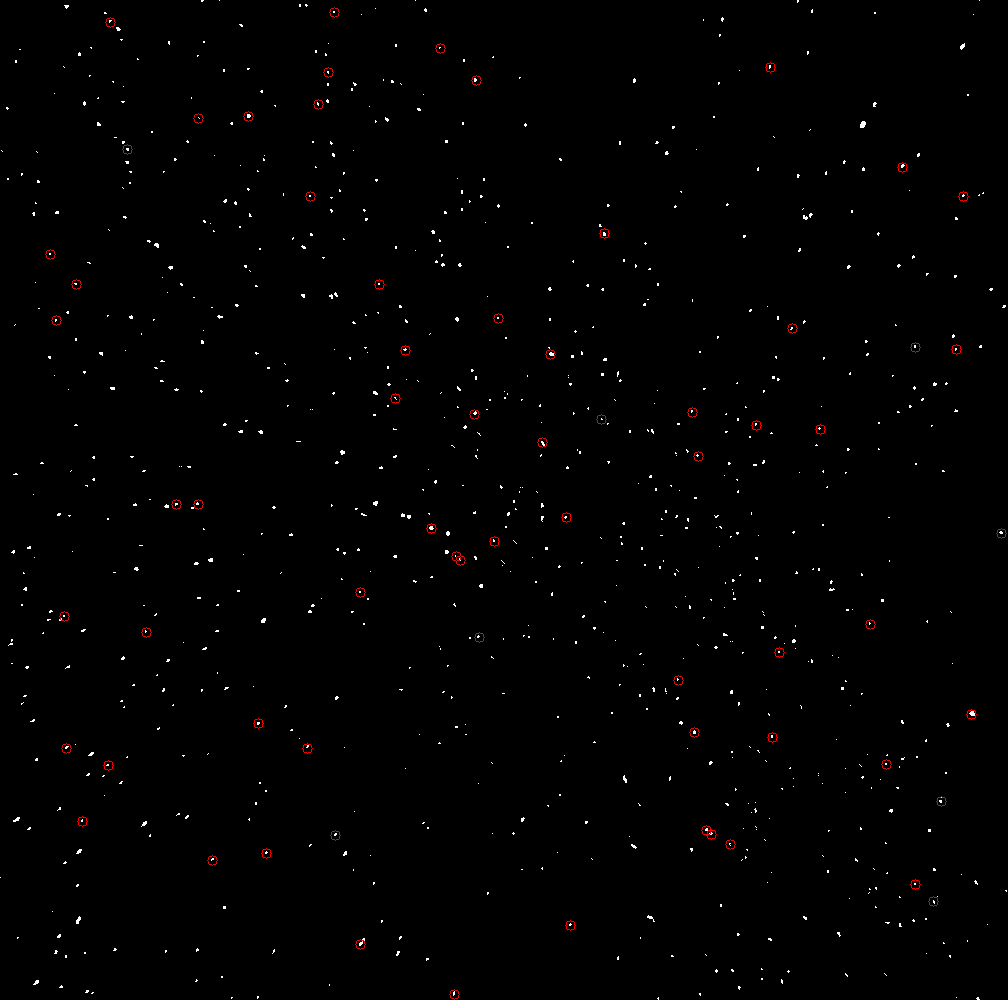
\includegraphics[width=\locateimgsize]{images/locate/4d-ptv.png}}
	\caption{\centering 4d-ptv's result}
	\label{fig:locate:fourdptv}
\end{figure}
